Exemple de texte cité \cite{Hambley}.\\
Exemple de note de bas de page\footnote[1]{hey now, you're a rockstar, get the show on get paid.}.

\subsection{Exemple d'équation}
  \begin{align}
    V &= RI \\
    2V &= 2RI \\
    V = RI \label{eq:notaligned}
  \end{align}
Comme on peut le constater, l'équation \ref{eq:notaligned} n'est pas alignée sur l'égalité.

% https://en.wikibooks.org/wiki/LaTeX/Tables
\subsection{Exemple de tableau}
  \begin{table}[H]
    \begin{center}
      \caption{Exemple de tableau}
      \begin{tabular}{l | c p{3cm}} 
        \hline
        \textbf{Colonne à gauche} & \textbf{Colonne centrée} & \textbf{Colonne justifiée} \\ [0.75ex] 
        \hline\hline
        Ligne 1 & taille dynamique & taille prédéfinie avec retour de ligne\\
        Ligne 2 & & \\
        Ligne 3 & & \\
        Ligne 4 & & \\
        Ligne 5 & & \\ [1ex]
        \hline
      \end{tabular}
    \end{center}
  \end{table}

\subsection{Exemple de graphique}
  \begin{figure}[H]
    \centering
    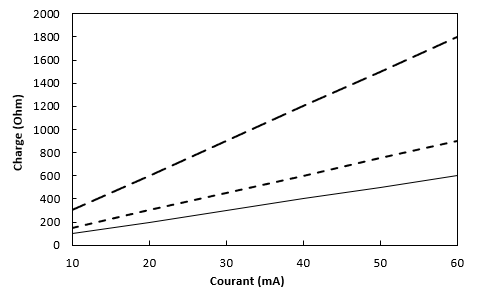
\includegraphics[scale=1]{Images/Graph.png}
    \caption{Exemple de graphique}
    \label{fig:Graph}
  \end{figure}

\subsection{Exemple d'histogramme}
  \begin{figure}[H]
    \centering
    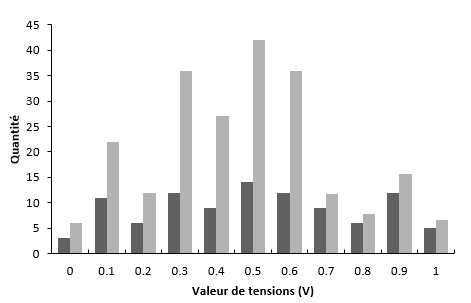
\includegraphics[scale=1]{Images/Histogram.png}
    \caption{Exemple d'histogramme}
    \label{fig:Histogram}
  \end{figure}
